

\section{Motifs}\label{sec:motifs}

Non-random connectivity in local cortical circuits extends well beyond
specific connection probability in neuron pairs: As one of their main
results, \textcite{Song2005} report a characteristic occurrence of
motifs of three neurons, while \textcite{Perin2011} find patterns in
the number of connections appearing in clusters of up to 8
neurons. Motifs have been shown to have a significant influence on
network dynamics, with patterns affecting dynamical
correlations \parencite{Pernice2011} and network
synchrony \parencite{Zhao2011}.

Finding no correlation between two-neuron connection probabilities and
anisotropy in connectivity prior, does anisotropy influence the
occurrence of neuron motifs? In this section we analyze higher order
connectivity in the different network types and observe a surprisingly
strong impact of anisotropy on patterns of connected neurons,
promoting the concept as an underlying principle for non-random
network connectivity.



\subsection*{Three-neuron patterns}

We first investigate the occurrence of three-neuron patterns in
an\-iso\-tro\-pic networks. \textcite{Song2005} reported a
characteristic, highly non-ran\-dom motif distribution of pyramidal
cells in the rat's visual cortex layer 5, a result later confirmed by
\textcite{Perin2011} in their experiment in the rat's somatosensory
cortex layer 5. Repeating the experiment \textit{in silico} for the
different networks subject to this study, we find similar,
characteristic motif distributions strongly influenced by anisotropy
in connectivity.

There are 13%
%------------------------------------
\footnote{%
  There are 16 non-isomorphic simple directed graphs with 3
  nodes. Three of those graphs are unconnected \parencite[cf. ][%
  N. J. A. Sloane. The On-Line Encyclopedia of Integer Sequences,
  http://oeis.org. Sequence
  \href{http://oeis.org/A000273}{A000273}]{Davis1953}.%
} %
%-------------------------------------
non-isomorphic 3-motifs in simple directed graphs. In reference to Song et al.'s result, the patterns
are labeled 4 to 16, \vspace{-0.2cm}
\begin{figure}[H]
  \centering
  \begin{overpic}[width=0.95\linewidth]{%
    plots/4839ce41_motifs_cropped.pdf}
  \put(100,0.2){.} 
  \end{overpic}
\end{figure}
\vspace{-0.8cm} Let $X$ be a random variable that maps three random
vertices $v_1 \neq v_2 \neq v_3$ in a graph $G$ to the $n \in
\{4,5,\dots,16\}$ labeling the isomorphism class of the full subgraph
with vertex set $\{v_1,v_2,v_3\}$ in $G$ as above if the subgraph is
connected, and let $X$ map to $n=0$ otherwise. A first idea of how to
compute the distribution of $X$ is by inferring the probabilities of
motif occurrence from the two-neuron connection probabilities from
Section~\ref{sec:two_neuron}. In anisotropic networks we found that
the probabilities of occurrence are 
\begin{align*} 
  p_u & = 0.791336     &&\text{for unconnected pairs,}     \\
  p_s & = 0.184151     &&\text{for single connections and} \\
  p_r & = 0.024513     &&\text{for reciprocal connections.}
\end{align*}
From these we may, for example, calculate the probability of
occurrence for motif 8, 
\[
  \mathbf{P}(X=8) = 6\, p_{u} p_{s} p_{r},
\]
where the factor 6 is determined by the number of different
\textit{labeled} graphs belonging to the isomorphism class. The
distribution of $X$ for the remaining motifs is given by \\
%
\smallskip
%
\begin{minipage}{\linewidth}
  \begin{minipage}[c]{0.32\textwidth}
    \begin{align*}
      % \mathbf{P}(X=1) &    =   p_u^3  \\
      % \mathbf{P}(X=2) &    =   6 p_u p_u p_s\\
      % \mathbf{P}(X=3) &    =   3 p_u p_u p_r\\
      \mathbf{P}(X=4) &    =   3 p_s^2 p_u\\
      \mathbf{P}(X=5) &    =   3 p_s^2 p_u\\
      \mathbf{P}(X=6) &    =   6 p_s^2 p_u\\
      \mathbf{P}(X=7) &    =   6 p_s p_u p_r
    \end{align*}
  \end{minipage}%
  \begin{minipage}[c]{0.32\textwidth}
    \begin{align*}
      \mathbf{P}(X=\,\,\,9) &    =   3 p_r^2 p_u\\
      \mathbf{P}(X=10) &   =   6 p_s^3   \\
      \mathbf{P}(X=11) &   =   2 p_s^3    \\
      \mathbf{P}(X=12) &   =   3 p_s^2 p_r
    \end{align*}
  \end{minipage}%
  \begin{minipage}[c]{0.32\textwidth}
    \begin{align*}
      \mathbf{P}(X=13) &   =   6 p_s^2 p_r\\
      \mathbf{P}(X=14) &   =   3 p_s^2 p_r\\
      \mathbf{P}(X=15) &   =   6 p_s p_r^2\\
      \mathbf{P}(X=16) &   =   p_r^3.
    \end{align*}
  \end{minipage}  
\end{minipage}

\begin{figure}[H]
  \centering
  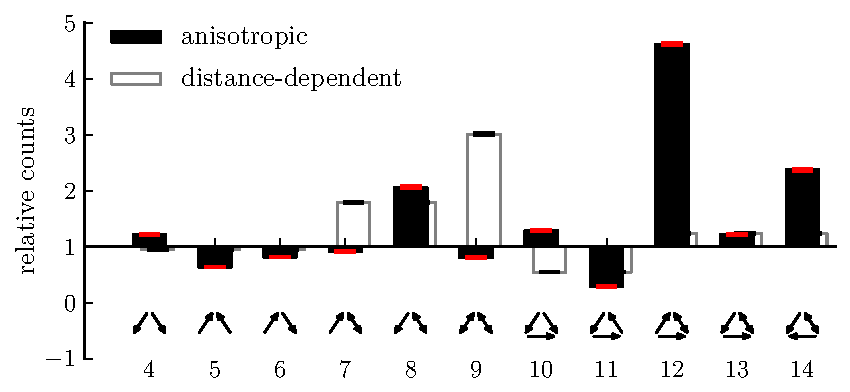
\includegraphics[width=0.95\linewidth]{%
    plots/4839ce41_aniso_dist.pdf}
  \captionsetup{skip=8pt}
  \caption{\textbf{Relative occurrence of three-neuron patterns}
    Extracting the counts of three-node motifs in anisotropic (filled
    bars) and distance-dependent networks (unfilled bars), the
    quotient of the obtained count with the number of occurrences
    expected from the two-neuron connection probabilities in the
    networks (cf. Section~\ref{sec:two_neuron}) shows the over- and
    underrepresentation of specific motifs in the network (red and
    black errorbars are SEM). In anisotropic networks pattern 12, for
    example, appears around five times more often than we would expect
    from the occurrence two-neuron connections. The relative counts
    for anisotropic networks resemble the findings of
    \textcite{Song2005} and differ significantly from the counts in
    distance-dependent networks, implying that anisotropy has a strong
    influence on the relative occurrence of three-neuron
    patterns. (\smtcite{4839ce41}) }
  \label{fig:3motif_single}
\end{figure}

Does this distribution accurately reflect the occurrences of
three-neuron motifs in anisotropic or even distance-dependent
networks? Here we take the distribution \marginpar{distribution from
  neuron-pairs as reference} determined from the two-neuron
probabilities as a reference to analyze occurrences of three-neuron
motifs in our sets of sample graphs. Counting the occurrences of
patterns in we find that there are significant over- and
underrepresentations in anisotropic as well as distance-dependent
networks, relative to our expectation
(\autoref{fig:3motif_single}). We find, for example, that in
anisotropic graphs pattern 12 occurs almost 5 times as often as we
would have expected from the two-neuron probabilities, whereas
the counts for pattern 11 only make up less than $30\%$ of the
occurrences expected.  

\begin{figure}[H]
  \centering
  \begin{overpic}[width=0.95\linewidth]{%
      plots/4839ce41_aniso_rew.pdf}
    \put(2.2,40){\small \textbf{A}} 
  \end{overpic}
  \begin{overpic}[width=0.95\linewidth]{%
      plots/4839ce41_tanfit_rew.pdf}
    \put(2.2,40){\small \textbf{B}}
  \end{overpic}
  \vspace{0.4cm}

  \makebox{%
    \hspace{1.208cm}%1.23
    \begin{overpic}[height=3.6cm]{%
        plots/4839ce41_motif15.pdf}
      \put(-10.8,45){\small \textbf{C}}
      \put(32.3,44.9){\small 15}
      \put(40,42.9){
\includegraphics[width=0.5cm]{img/misc/song_motif_15.pdf}}
    \end{overpic} 
    \hspace{0.19cm}
    \begin{overpic}[height=3.6cm]{%
        plots/4839ce41_motif16.pdf}
      \put(54,83){\small 16}
      \put(68,79){
\includegraphics[width=0.5cm]{img/misc/song_motif_16.pdf}}
    \end{overpic} 
  }%

  \captionsetup{skip=8pt}
  \caption{\textbf{Three-neuron motif occurrence in different network
      types} \textbf{A)} Comparing counts in anisotropic sample graphs
    with their rewired counterparts. \textbf{B)} Three-neuron motifs
    occurrence in tuned anisotropic networks
    (cf. Section~\ref{sec:tuned_networks}) with their rewired
    counterparts. For this two-neuron connection probabilities were
    extracted as in Section~\ref{sec:two_neuron} and motif
    probabilities were calculated analogously to anisotropic
    networks. \textbf{C)} Relative counts for the high edge count
    motifs 15 and 16 for different network types, errorbars
    SEM. (\smtcite{4839ce41}) }
  \label{fig:3motif_full}
\end{figure}

Comparing the relative counts for motifs in anisotropic graphs with
those in comparable distance-dependent networks, we
\marginpar{anisotropy strongly affects 3-motif
  occurrence}identify a strong influence of anisotropy in connectivity
on three-neuron motif occurrence (\autoref{fig:3motif_single}). In
their experiments, Song et al.\ and Perin et al.\ find an
overrepresentation of motifs 4, 10, 12 and 14. In anisotropic networks
increased counts of motifs 4, 8, 10, 12, 13 and 14 were
recorded. However, motifs 8 and 13 are overrepresented in
distance-dependent networks as well, leaving the reported motifs 4,
10, 12 and 14 as motifs that are overrepresented due to anisotropy. To
analyze this effect closer, we also compare three-neuron counts before
and after rewiring in anisotropic networks
(\autoref{fig:3motif_full}).

Considering motif occurrences in anisotropic as well as tuned
anisotropic networks, we once again confirm the overrepresentation of
motifs 4, 10, 12 and 14. However, increased counts of pattern 4 are
observed in the rewired networks as well, leading to the conclusion
that increased occurrence in this motif is only implicitly affected by
anisotropy. Motifs 10, 12 and 14 however show significant
overrepresentation even over their rewired counterparts in anisotropic
as well as in tuned anisotropic networks.

The overall motif distribution shows itself stable under changes in
the distance-dependency with the notable exception of motif 9, that
shows underrepresentation only in anisotropic but not in tuned
anisotropic or any distance-dependent network type. Analyzing the
occurrences of motifs 15 and 16 with a high edge counts
(\autoref{fig:3motif_full} C) we find that anisotropy has strong
influence on both motifs, with motif 15 being significantly
overrepresented in anisotropic networks. Motif 16 shows a highly
increased occurrence in anisotropic networks, however tuning causes
the loss of this feature in the network connectivity.

Summarizing the above observations, we find that \marginpar{results
  summary} anisotropy in connectivity induces increased occurrence of
motifs 10, 12, 14 and 15 in the network, reflecting experimental
results in the rat's cortex.  While over- and underrepresentation
observed in local cortical circuits can be indirectly linked to
anisotropy for some motifs (4, 9), it does not accurately reflect
observed counts for other motifs (8) and shows instability under
manipulation of distance-dependency in some patterns (9, 16).



\subsection*{On motif occurrence in networks}

In obtaining and discussing the previous results, we closely followed
the approach described by \textcite{Song2005}. Here, relying on
analytical considerations, we submit these results to a critical
analysis and identify potential caveats when dealing with motif
distributions in distance-dependent networks.

For this consider for example the motifs 9, 15 and 16 as labeled
above. In distance-dependent networks we find that each of the
patterns is overrepresented, observing that the motifs occur about 3,
3 and 12 times more often than expected from the two-neuron connection
probabilities, respectively (\autoref{fig:3motif_single}). Thus, in
distance-dependent networks, triplets in which two of the pairs are
reciprocally connected appear more often than expected, regardless of
the connectivity in the third pair. This is surprising, as
probabilities for the first two neuron pairs in a triplet should be
independent and the probabilities of obtaining a certain connectivity
should reflect the product of two-neuron probabilities. The
overrepresentation found in these motifs may thus not necessarily be
an inherent feature of the network connectivity but rather an artifact
of triplet selection.

To analyze this further, we compute the relative probabilities of
occurrence for motifs 9, 15 and 16. Formulated differently, given a
triplet with two reciprocally connected pairs, what is probability of
connection in the third pair? For this we first find the probability
density function of the distance between a random neuron pair, given
that we know its connectivity, meaning the existence of either 0, 1 or
2 edges between the neuron. Let $X$ be the random variable mapping a
random neuron pair of neurons to the distance between then and $Y$ the
random variable mapping to the number of edges between the pair. By
the relation
\[
f_X(x \vert Y=n) = \frac{f_{X,Y}(x,n)}{\mathbf{P}(Y=n)},
\]
for $n=0, 1, 2$, the probability density function $f_X$ of the continuous variable
$X$ conditioned on the discrete variable $Y$, are then computed as the
quotients
%
\medskip
\begin{equation}
\begin{aligned}
  %
  f_X(x \vert Y=0)%
    & = \frac{f(x) (1-C(x))^2}%
            {\int_0^{\sqrt{2}} f(x) (1-C(x))^2 \, dx}%
     \\[1em]%
  %
  f_X(x \vert Y=1)%
    & = \frac{f(x) 2 C(x) (1-C(x))}%
             {\int_0^{\sqrt{2}} f(x) 2 C(x) (1-C(x)) \, dx}%
      \\[1em]%
  %
  f_X(x \vert Y=2)% 
    & = \frac{f(x) C(x)^2}
             {\int_0^{\sqrt{2}} f(x) C(x)^2 \, dx},
  %
\end{aligned}
\label{eq:cond_prob}
\end{equation}
%
where $f(x)$ is the probability density function of the distance
between two random in the unit square the found in
Theorem~\ref{theorem:distance_square} and $C(x)$ the
distance-dependent connectivity from
Theorem~\ref{theorem:distance_prof}. Values for the denominator in
Equation~\ref{eq:cond_prob} have already been determined in
Section~\ref{sec:two_neuron}. Evaluating the products in the
numerator, we find that the expected probability density function is
perfectly match by the distance distributions found in the simulated
distance-dependent network model (\smtcite{38c11969}):

\begin{figure}[H]
  \vspace{1.2cm}
  \centering
  \makebox[0.925\textwidth]{%
    \begin{overpic}[width=0.45\textwidth]{%
        plots/38c11969_y1.pdf}
      \put(44.5,45.2){\small$f_X(x \vert Y=1)$}
    \end{overpic}
    \hfill
    \begin{overpic}[width=0.45\textwidth]{%
        plots/38c11969_y2.pdf}
      \put(44.5,45.2){\small$f_X(x \vert Y=2)$}
    \end{overpic}
  }%
  % %\captionsetup{skip=7pt}
  % \caption{\textbf{Anisotropy increases variance of common input
  %    distribution} Recording common in-neighbor counts for random
  %   neuron pairs in tuned anisotropic networks and their rewired
  %   versions reveals increased variance in networks with a high degree
  %   of anisotropy. \textbf{A)} Common in-neighbor distribution for
  %   original tuned anisotropic networks ($\eta = 0$, blue) and rewired
  %   versions with $\nicefrac{1}{4}$ of all edges rewired ($\eta =
  %   0.25$, red) and completely rewired ($\eta =1 $, green).
  %   (\smtcite{5841710e}) \textbf{B)} Variance of the common
  %   in-neighbor distributions declines with increasing rewiring factor
  %   $\eta$; highest variance is found in networks with the highest
  %   degree of anisotropy ($\eta = 0$). Errorbars SEM. (\smtcite{ffcefe9b})}
  % \label{fig:co} %??
\end{figure}

Consider then a triplet with vertices $v_1, v_2$ and $v_3$, the pairs
$(v_1,v_2)$ and $(v_1, v_3)$ being reciprocally connected. With the
density function $f_X(x|Y=2)$ we then have a distribution for the
distances $x = d(v_1, v_2)$ and $y = d(v_1,v_3)$. In the triangle
spanned by the positions of the vertices, the distance $z=d(v_2,v_3)$
is then determined by the angle $\theta$ between $x$ and $y$:


\begin{minipage}{\textwidth}
  \centering
  \begin{overpic}[width=0.4\textwidth]{%
      tikz/circle_connectivity.pdf}
  \end{overpic}
  \medskip
\end{minipage}
%
By the law of cosines, between $x, y, z$ and $\theta$ we have the relation 
\begin{align}
\label{eq:law_cosine}
z = \sqrt{ x^2 + y^2 - 2xy \cos \theta}.
\end{align}
From this we can, extensively using Lemma~\ref{lem:
  lemma:transform_random_variable}, calculate the probability density
of $z$ in the triplet $(v_1, v_2, v_3)$ from the densities $f_X(x
\vert Y=2)$ of $x$ and $y$, similar to the proof of
Theorem~\ref{theorem:distance_square}. Here, however, it suffices to
find the expected value of $z$. The expected values for $x$ and $y$
are
\[
r:=\mathbf{E}[x] = \mathbf{E}[y] =  \int_{0}^{\sqrt{2}} x f_X(x|Y=2) \, dx.
\]
Finding the expected value of $z$ is then the well known problem of
determining the length of a chord between two random points on the
circle \parencite[cf.][]{MathWorld_Circle}. For $x,y=r$,
Equation~\ref{eq:law_cosine} becomes% 
%
\begin{align*}
z(\theta) = r \sqrt{2 - 2 \cos \theta} =2 r \abs{\sin \frac{\theta}{2}}.
\end{align*}%
\marginpar{\vspace{-1.94cm}\\ half-angle formula,\\  \textcite{Abramowitz_Handbook}}%
Using the symmetry of the problem, we then find the expected value for $z$
by integration,  
\begin{align*}
\mathbf{E}[z] & = \int_0^{2\pi} \frac{1}{2\pi} z(\theta) \, d\theta \\ 
              & = \int_0^{2\pi} \frac{r}{\pi} \abs{\sin
                \frac{\theta}{2}} \, d\theta \\
              & =  \frac{2r}{\pi} \int_0^{\pi} \sin
                \frac{\theta}{2} \, d\theta  = \frac{4r}{\pi}.
\end{align*}

With the expected distance $z$ we can the finally calculate the
relative probabilities to obtain either motif 9, 15 or 16 from the
distance-dependent connectivity profile $C(x)$. If $Z$ is the random
variable mapping given a triplet $(v_1, v_2, v_3)$ with reciprocal
connections between $v_1$ and $v_2$, as well as $v_1$ and $v_3$ to the
labels of the possible motifs 9, 15 or 16 describing the triplet, the
distribution is (Mathematica~\ref{mathematica:motif})
\begin{equation}
  \label{eq:rel_prob}
  \begin{aligned}%
    \mathbf{P}(Z=\,\,9\,) & =  \left(1-C(\mathbf{E}[z])\right)^2 && = 0.697628  \\
    \mathbf{P}(Z=15) &= 2\,C(\mathbf{E}[z])\, (1-C(\mathbf{E}[z]))&& = 0.275227   \\
    \mathbf{P}(Z=16) &=  C(\mathbf{E}[z])^2 && = 0.0271455.
  \end{aligned}%
\end{equation}

What relative occurrences would be expect from the two-neuron
connection probabilities? For this we take the probabilities to find
motifs 9, 15 and 16 under all motifs,  
\begin{align*}
      \mathbf{P}(X=9)    =   3 p_r^2 p_u, \quad\,       \mathbf{P}(X=15)   =
      6 p_s p_r^2, \quad\, \mathbf{P}(X=16)   =   p_r^3,
\end{align*}
and normalize the probabilities by their sum. Building the quotient of
the calculated relative probabilities $\mathbf{P}$ from (\ref{eq:rel_prob}) with
the expected relative frequency $\tilde{F_2}$, inferred from two-neuron connectivity, we
find the relative overrepresentation in the family of triplets with
two reciprocal connections.

\begin{minipage}{0.8\linewidth}
  %
  \vspace{0.9cm}

  \hspace{1cm}
  \begin{overpic}[width=0.65cm]{%
      img/misc/song_motif_09.pdf}
    \put(-80,25){9}
    \put(360,165){$\tilde{F_2}$}
    \put(710,165){$\nicefrac{\mathbf{P}}{\tilde{F_2}}$}
    \put(1060,165){$ \nicefrac{k\mathbf{P}}{\tilde{F_2}}$}
    \put(1410,165){$F_2$}
    % 
    %
    \put(270,25){$0.677625$}
    \put(680,25){$1.0295$}
    \put(1045,25){$3.2408$}
    \put(1365,25){$2.9852$}
    %
  \end{overpic}
  \bigskip
  \vfill
  \hspace{1cm}
  \begin{overpic}[width=0.65cm]{%
      img/misc/song_motif_15.pdf}
    \put(-100,25){15}
    \put(270,25){$0.315379$}
    \put(680,25){$0.8727$}
    \put(1045,25){$2.7471$}
    \put(1365,25){$3.2810$}
  \end{overpic}
  \bigskip
  \vfill
  \hspace{1cm}
  \begin{overpic}[width=0.65cm]{%
      img/misc/song_motif_16.pdf}
    \put(-100,25){16}
    \put(270,25){$0.006997$}
    \put(680,25){$3.8797$}
    \put(1015,25){$12.2126$}
    \put(1336,25){$12.9001$}
    \put(1080,-120){(label: \smtcite{b5e4ed3e})}
  \end{overpic}
  %
  \vspace{0.9cm}
\end{minipage}

We note that amongst triplets with two reciprocal connections, motif
16 appears about four times as often as expected, while motifs 9 and
15 are not significantly over- or underrepresented. How do these
numbers relate to the absolute overrepresentation $F_2$ amongst all
three-motifs? We find that triplets with two reciprocal connections
appear $k=3.1478$ as often amongst all three-motifs as expected
(\smtcite{b5e4ed3e}); multiplying the quotient
$\nicefrac{\mathbf{P}}{\tilde{F_2}}$ with $k$ then yields an absolute
overrepresentation as found in the simulated distance-dependent
networks.

In distance-dependent networks, independence in the connectivity
\marginpar{summary \& discussion}of the first two neuron pairs was expected. From
our simulations, however, we clearly find that all triplets with at
least two reciprocally occur more frequently than expected. This is
due to boundary effects - neurons located close to the border or even
a corner have drastically different distribution of distances to all
other neurons as node located close to the center. Thus, rectifying
for this bias, the \enquote{true} overrepresentation was calculated in
(\ref{eq:rel_prob}), finding only motif 16 with an increased
occurrence relative to the expectation.

Fortunately, results in anisotropic networks remain unaffected by this
problem. As only statements relative towards rewired or
distance-depen\-dent networks were made, both containing this bias,
overrepresentation due to anisotropy could still be accurately
identified. Song et al.'s three-motif distribution also does not
immediately show this problem. While, for example, motifs 9, 15 and 16
are all reported as overrepresented, it is well in the error margin of
their experiment to have triplets with at least two reciprocal
connections appearing overall as expected.  However, the analysis
shown here may well be important for further studies in brain
connectivity, testing results against potential biases, or, gaining
new insights on neuronal connectivity, finding without doubt that such
overrepresentations do occur.

 

% Thus, while motif 9 and 15 appear inrelatively among three-motifs with
% two reciprocal connetions, motif 16 appears four times as often. This
% result is immediately confirmed by our computational results, finding
% that triplets with appear 3 in general, and .


% The \enquote{true} overrepresentation may thus only be present in
% motif 16, appearing four more times as expected



%  How does this affect the results described
% above? As distant-dependent networks are clearly 


% %\newpage

\subsection*{Edge counts in neuron clusters}

In motifs consisting of 3 to 8 neurons, \textcite{Perin2011} reported
a striking statistic from their experiment with pyramidal cells in the
rat's somatsosensory cortex, layer 5: Counting the number of edges
appearing in a cluster of $n$ neurons, they find that clusters with
relatively high edge counts appear significantly more often than
expected from the network's distance-dependent connection
probabilities alone. Do anisotropic networks exhibit a similar
feature?

\begin{figure}[h!]
  \centering
  \begin{overpic}[width=0.95\linewidth]{%
      plots/76cc6fa0.pdf} 
    \put(3.2,43){\small \textbf{A}}
  \end{overpic}
  \begin{overpic}[width=0.95\linewidth]{%
    plots/7c826e10.pdf} 
    \put(3.2,43){\small \textbf{B}}
  \end{overpic}
  \begin{overpic}[width=0.95\linewidth]{%
    plots/54329cf4.pdf} 
    \put(3.2,43){\small \textbf{C}}
  \end{overpic}
  \captionsetup{skip=10pt}
  \caption{\textbf{High edge counts are overrepresented in networks
      with anisotropy} Normalized difference between number of edges
    in clusters of 6, 8 and 12 randomly selected neurons in
    anisotropic networks and rewired networks shows an
    overrepresentation of high edge counts in networks with anisotropy
    in connectivity. Errorbars SEM. (\smtcite{76cc6fa0},
    smtcite{987992b0}, \smtcite{54329cf4})}
  \label{fig:perin6to12}
\end{figure}

Recruiting the collection of sample graphs once again we analyze the
occurrence of edge counts in clusters of $n$ neurons in the different
network types. In the main process, after randomly sampling $n$
pairwise different vertices $S_n$, the motif $H$ in $G$ with vertex
set $V(H) = S_n$ is identified and its number of edges $\abs{E(H)}$ is
recorded. Repeating this sufficiently often (order $10^6$) we obtain
edge counts for clusters of 6,8 and 12 neurons in the anisotropic- and
tuned anisotropic networks as well as in their rewired
counterparts. Then, showing the difference between counts in the
anisotropic networks and counts in the rewired networks, normalized by
the rewired counts, we identify an overrepresentation of high edge
counts in the neuron similar to Perin et al.\
(\autoref{fig:perin6to12}).

In anisotropic networks an overrepresentation of high edge counts is
found consistently through clusters of 6, 8 and 12 neurons, with the
highest counts appearing up to four times as often as expected. Low
edge counts occur less frequently than expected and an increasing
number of connections shows an oscillation around the
expectation. These findings are consistent with the report of Perin et
al, which however indicates a higher maximal overrepresentation in
clusters of 8 neurons. 

Tuning the network's distance-dependency appears to not affect the
overrepresentation as edge counts in anisotropic and tuned
an\-iso\-tro\-pic essentially match
(\autoref{fig:perin6to12}). Anisotropy in connectivity therefore
presents itself as an important factor in the occurrence of increased
high edge counts in cortical networks, possibly fully reflecting the
findings of Perin et al., as the overrepresentation effect is found to
be even stronger when comparing edge counts to distance-dependent
networks as opposed to rewired versions (\autoref{fig:perin_rew_dist}).


\begin{figure}[H]
  \centering
  \begin{overpic}[width=0.95\linewidth]{%
      plots/7c826e10_dist_rew_comp.pdf} 
    %\put(3.2,43){\small \textbf{A}}
  \end{overpic}
  \captionsetup{skip=8pt}
  \caption{\textbf{Stronger overrepresentation of clusters with high
      edge counts with distance-dependent networks as reference}
    Showing the occurrence of edge counts in clusters of 8 random
    neurons, we find that the overrepresentation of motifs with high
    edge counts is stronger when taking distance-dependent networks as
    a reference as opposed to rewired networks. (\smtcite{7c826e10}) }
  \label{fig:perin_rew_dist}
\end{figure}











%%% Local Variables: 
%%% mode: latex
%%% TeX-master: "../dplths_document"
%%% End: 
